\chapter{Posizione}
\label{sec:posizione}

Una camera acquisisce un'immagine catturando la luce proveniente dalla scena in un sensore posto dietro un'apertura, normalmente controllata da un otturatore.
Per focalizzare i raggi di luce sul sensore è utilizzata una lente.
Queste lenti introducono una distorsione radiale nell'immagine catturata, che dipende dalla curvatura della lente.
In alcuni casi tale distorsione è particolarmente intensa, ed è necessario correggerla prima di affrontare la distorsione prospettica, ma nella maggioranza dei casi questa non è significativa e può essere ignorata.

\begin{figure}
    \centering
    \begin{subfigure}{.49\textwidth}
        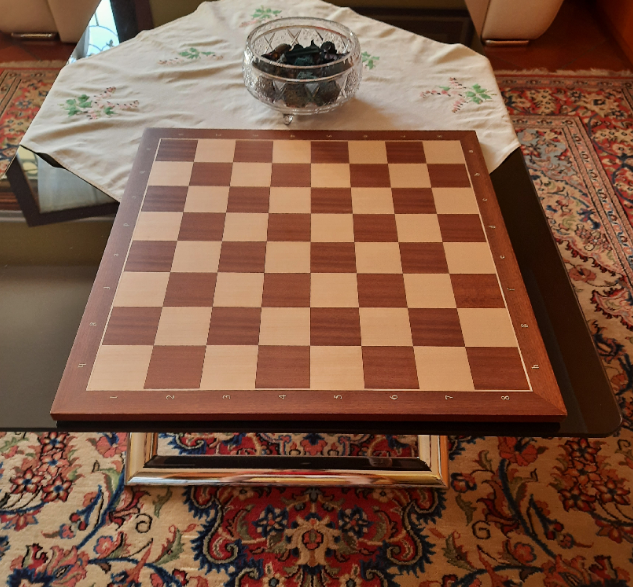
\includegraphics[width=\textwidth]{images/persp1.png}
    \end{subfigure}
    \hfill
    \begin{subfigure}{.49\textwidth}
        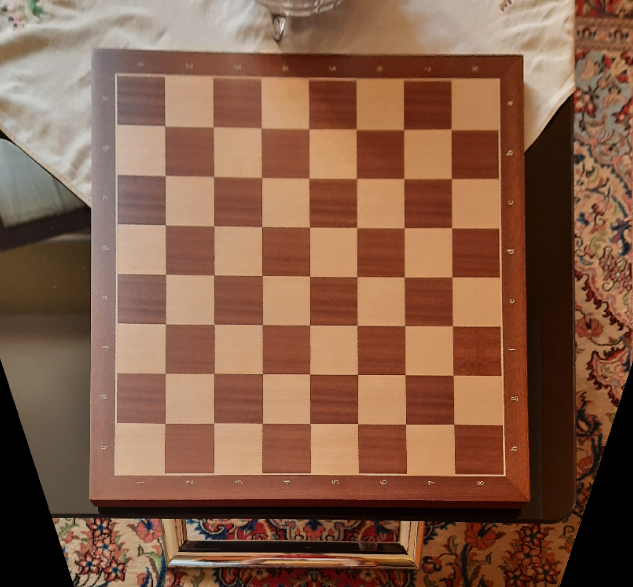
\includegraphics[width=\textwidth]{images/persp2.png}
    \end{subfigure}
    \caption{Esempio di correzione della distorsione prospettica}
    \label{fig:projcorrected}
\end{figure}

L'operazione di cattura dell'immagine può quindi essere modellata come proiezione dello spazio reale su un piano immagine, in cui i raggi di luce corrispondono alle linee di proiezione e in cui la camera corrisponde al punto in cui le linee di proiezione convergono.
Per la correttezza del nostro modello è importante mantenere il rapporto tra lunghezza focale e la dimensione dei pixel, e la posizione dell'immagine rispetto all'asse della camera.
Non è quindi necessario che la distanza tra immagine e camera nel nostro modello corrisponda a quella tra il sensore e la lente nella realtà, ma può essere scelta in modo da ottenere misure più agevoli per i calcoli.
Comunemente la lunghezza focale si esprime in pixel, e si sceglie come dimensione dei pixel 1 unita dello spazio reale.
Così facendo è possibile utilizzare qualsiasi unità di misura desiderata per la realtà senza dover modificare le coordinate dei punti dell'immagine.
Un'altra scelta comune per semplificare i calcoli è quella di porre l'origine degli assi delle coordinate al centro dell'immagine, orientare l'asse $x$ con le righe dell'immagine, l'asse $y$ con le colonne, e l'asse $z$ con l'asse ottico della camera, che è la linea che passa tra la camera e il centro dell'immagine (fig \ref{fig:camera coords}).

\begin{figure}
    \centering
    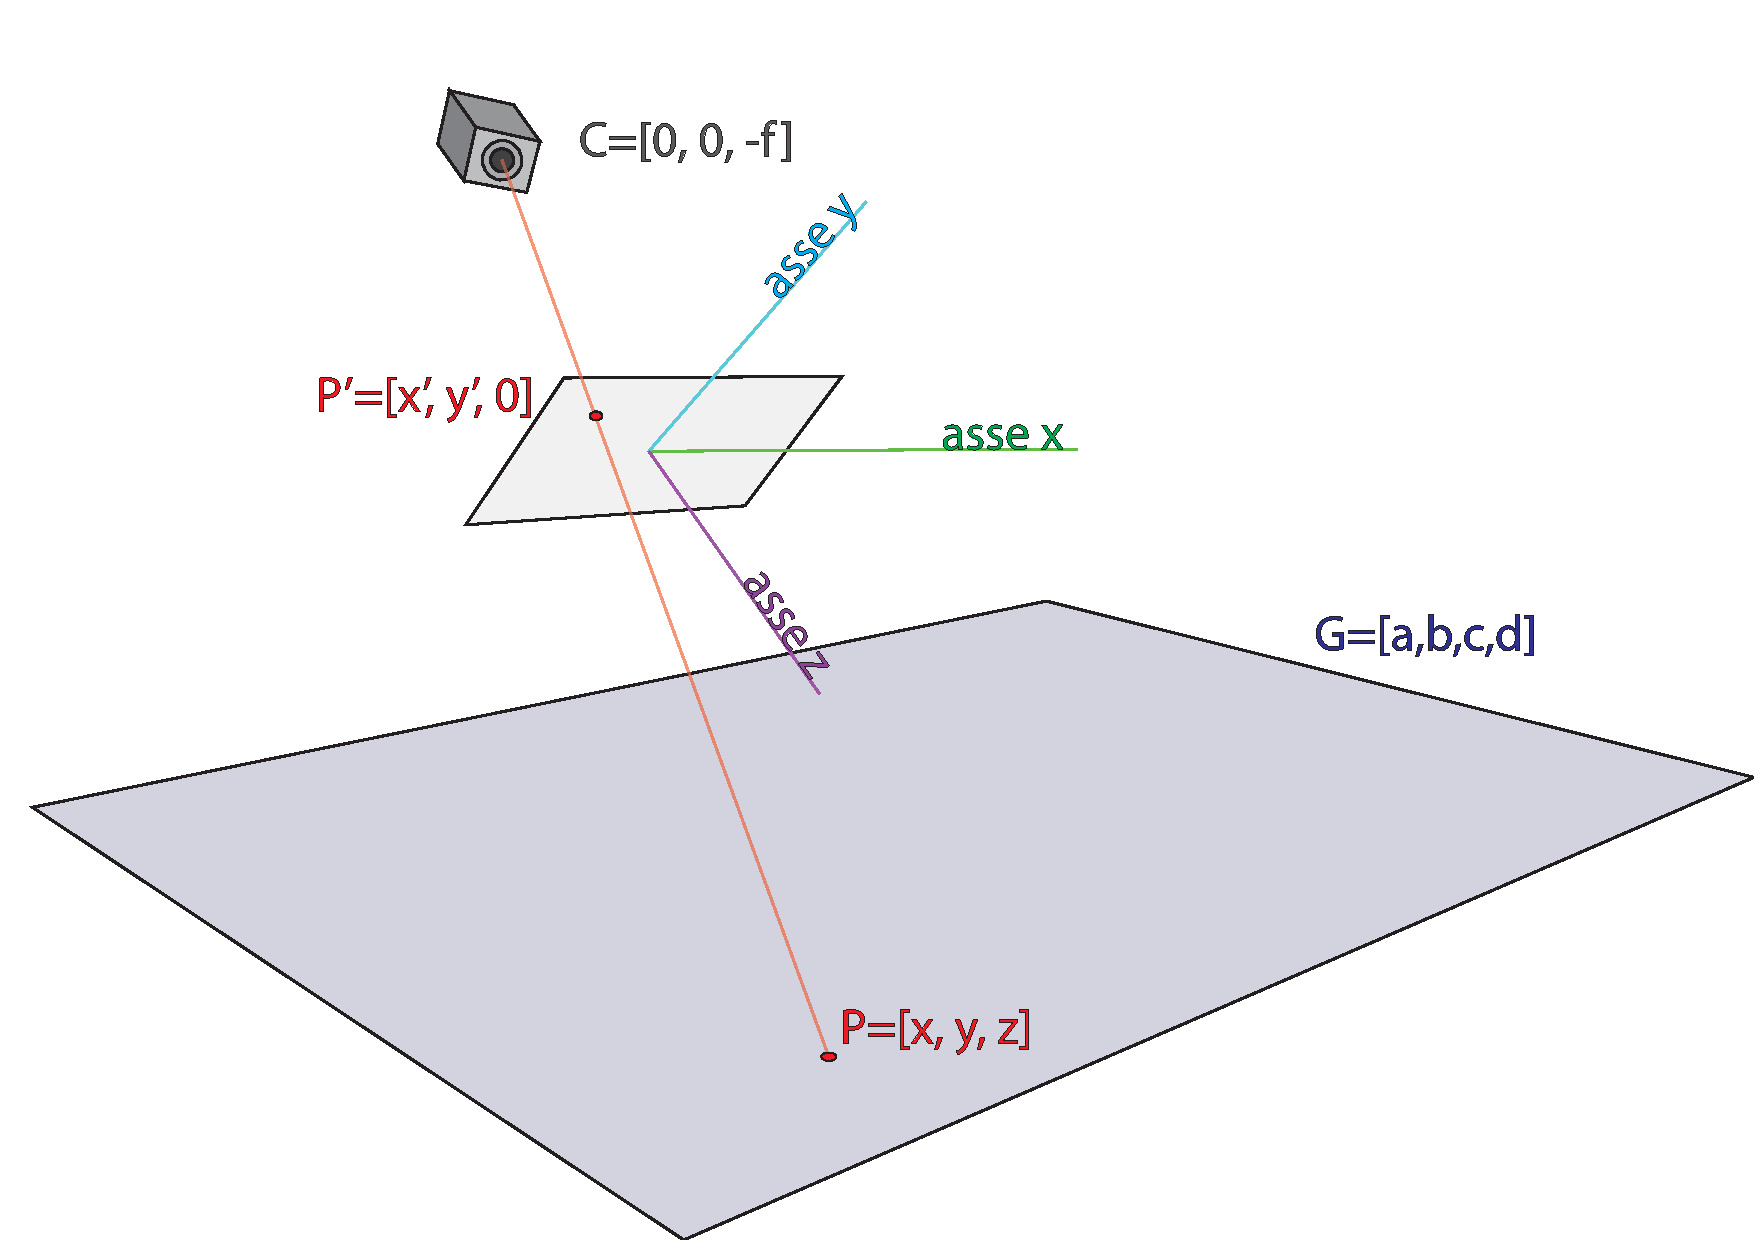
\includegraphics[width=\textwidth]{images/camera coords.pdf}
    \caption{Modello con coordinate}
    \label{fig:camera coords}
\end{figure}

Come espresso nella sezione \ref{sec:funzionalita-posizione} a noi interessa solamente ricorstruire ciò che accade sulla strada e ignoriamo il resto della scena.
Possiamo approssimare la strada con un piano, che chiamiamo piano stradale.
L'operazione che dobbiamo eseguire per correggere la distorsione prospettica si riduce così dalla proiezione da immagine a spazio reale tridimensionale a una proiezione da immagine a piano bidimensionale.
Questa operazione non è lineare in coordinate cartesiane, ma diventa lineare se si utilizzano coordinate proiettive omogenee, ed è quindi possibile definire una matrice lineare di trasformazione.

È possibile definire tale matrice direttamente, ma è anche possibile definirla come combinazione di trasformazioni.
Tutte le trasformazioni affini sono componibili in coordinate omogenee, ed abbiamo quindi accesso a traslazione, rotazione e scalatura, a cui aggiungiamo la trasformazione di proiezione.
La trasformazione di proiezione prende le coordinate di un punto sull'immagine e, date le coordinate del piano, restituisce la posizione reale del punto corrispondente al punto immagine.
Dato che le coordinate sono omogenee e non cartesiane, il punto immagine è espresso con 3 coordinate e il punto reale trovato con 4 coordinate.
La trasformazione di proiezione $P$ è rappresentata con la matrice \ref{eq:projmat}:
\begin{equation}
        \label{eq:projmat}
        P = 
        \begin{bmatrix*}[r]
            cf - d & 0      & 0   \\
            0      & cf - d & 0   \\
            -fa    & -fb    & -fd \\
            a      & b      & cf  \\
        \end{bmatrix*}
\end{equation}
Dove:
\begin{itemize}
    \item il piano stradale è caratterizzato dall'equazione $ax + by + cz + d = 0$, oppure dal vettore $[a, b, c, d]^T$
    \item la lunghezza focale della camera è $f$
\end{itemize}

La matrice di trasformazione completa $M$ è definita quindi dalla combinazione di trasformazioni in \ref{eq:projcombo}:
\begin{equation}
    \label{eq:projcombo}
    M = D \cdot T \cdot R \cdot P
\end{equation}
Dove:
\begin{itemize}
    \item $P$ è la matrice di proiezione dall'immagine al piano
    \item $R$ è la rotazione dalla normale del piano all'opposto della normale dell'immagine
    \item $T$ è la traslazione dall'origine del piano all'origine dell'immagine
    \item $D$ è la matrice 
    $
    \begin{bsmallmatrix}
        1 & 0 & 0 & 0 \\
        0 & 1 & 0 & 0 \\
        0 & 0 & 0 & 1 \\
    \end{bsmallmatrix}
    $
    che scarta la coordinata $z$ e ci riporta da 3 dimensioni a 2 dimensioni
\end{itemize}
Ricordiamo che le trasformazioni combinano da destra verso sinistra.
Una rappresentazione visiva della combinazione è in fig \ref{fig:tcombo}.

\begin{figure}[h]
    \centering
    \begin{subfigure}{.32\textwidth}
        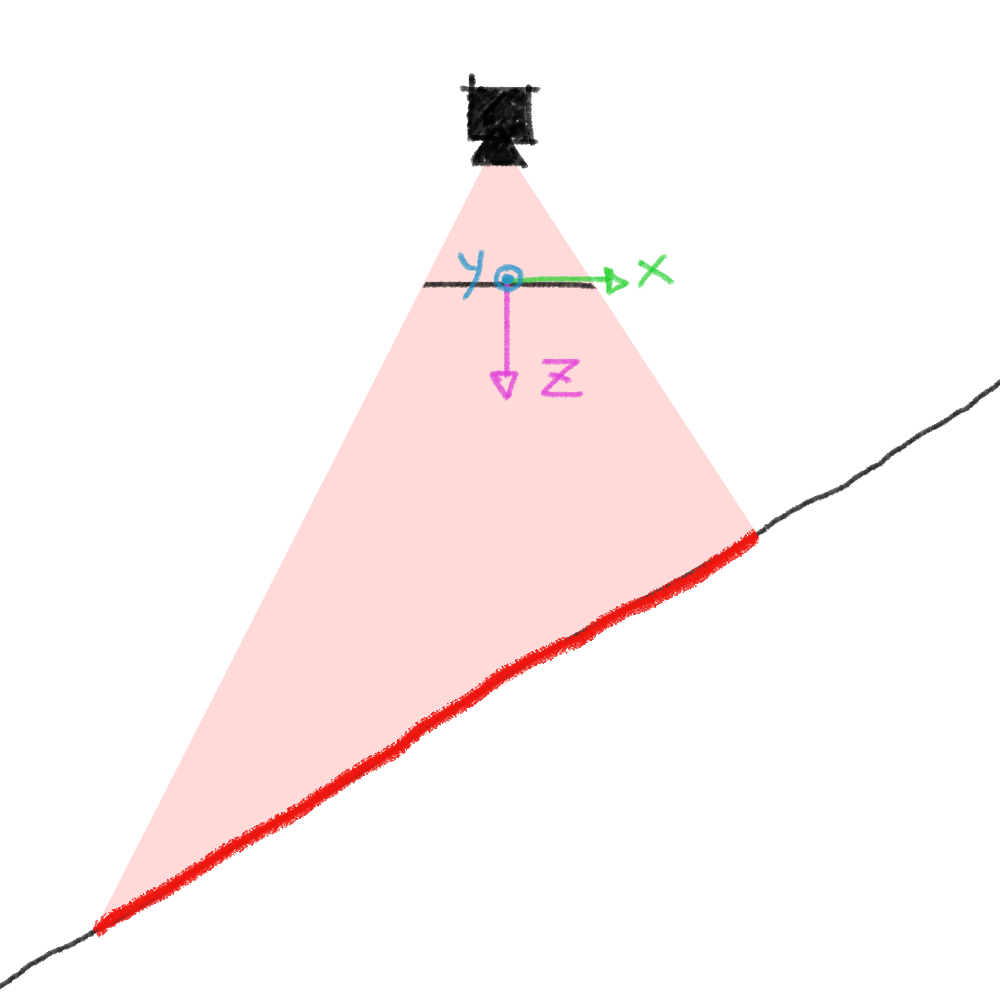
\includegraphics[width=\textwidth]{images/P.png}
        \caption{$P$}
    \end{subfigure}
    \hfill
    \begin{subfigure}{.32\textwidth}
        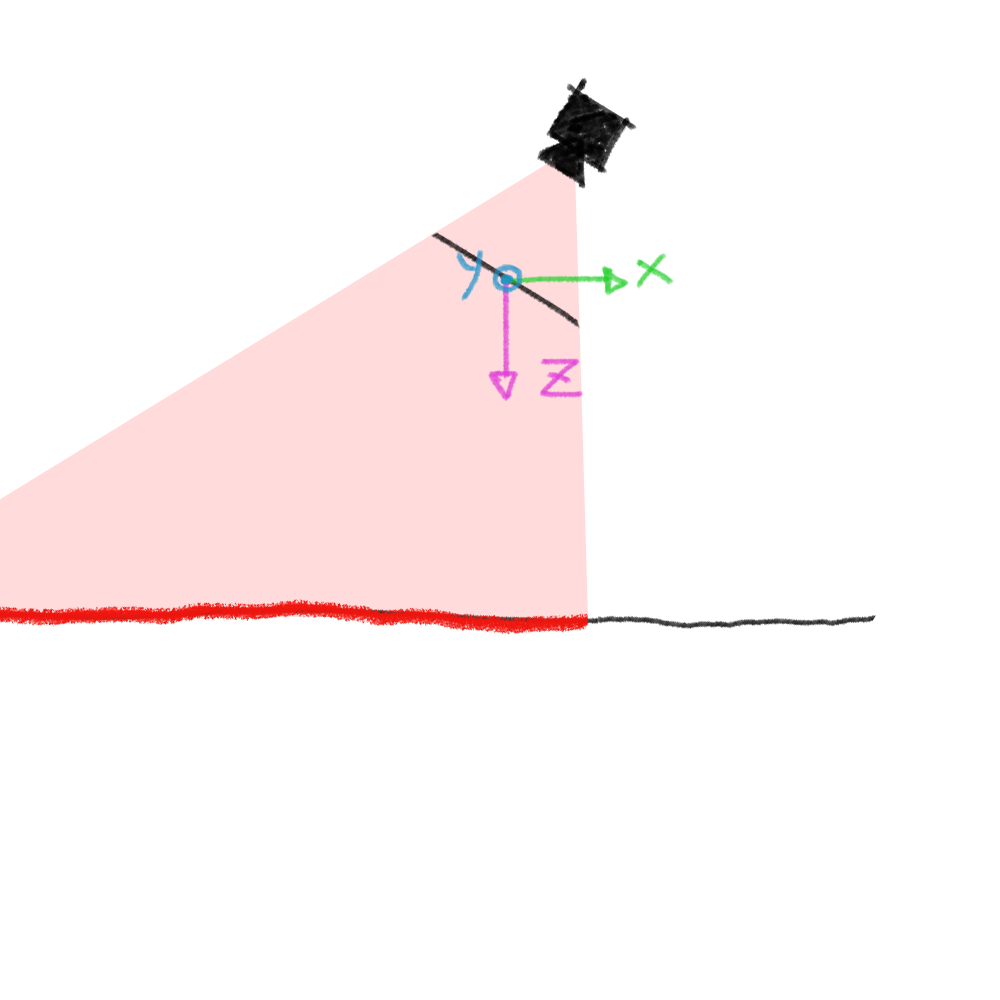
\includegraphics[width=\textwidth]{images/R.png}
        \caption{$R$}
    \end{subfigure}
    \hfill
    \begin{subfigure}{.32\textwidth}
        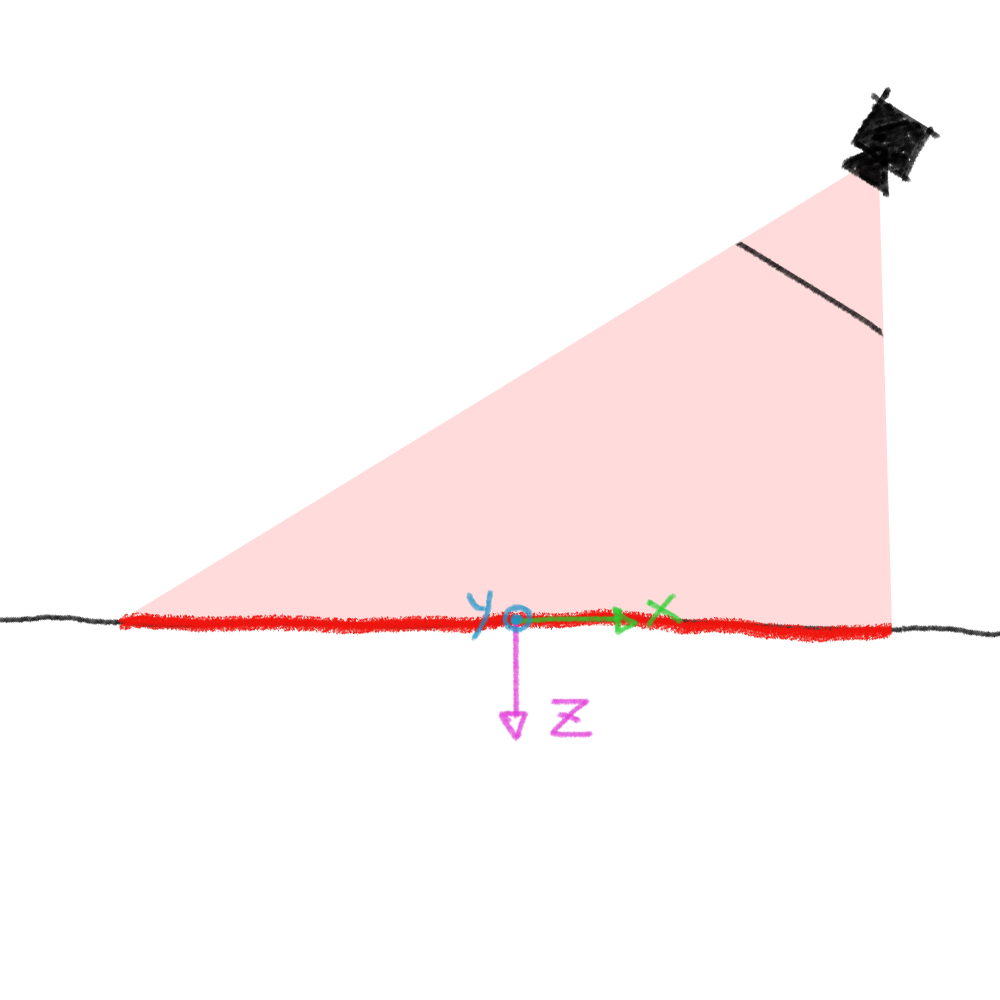
\includegraphics[width=\textwidth]{images/T.png}
        \caption{$T$}
    \end{subfigure}
    \caption{Trasformazione completa}
    \label{fig:tcombo}
\end{figure}

Diventa quindi possibile definire la matrice di correzione della distorsione prospettica in modo interattivo, manipolando la rotazione e la posizione della camera rispetto al piano stradale.
Possiamo infatti calcolare le coodinate del piano necessarie per $P$ partendo dal piano $[0, 0, 1, 0]$ (è il piano $z=0$) e applicando $R^{-1}$ e $T^{-1T}$ (la traslazione in coordinate proiettive si applica al piano mediante la trasposta della traslazione applicata ai punti).
In questo modo si può trovare una trasformazione soddisfacente, in cui le misure si avvicinano a quelle reali, senza i grandi costi implementativi richiesti dall'implementazione di un metodo automatico per la definizione del piano stradale.
Una volta definita la matrice di trasformazione il suo utilizzo risulta estremamente efficiente, in quanto si riduce a un prodotto matrice-vettore.

\begin{figure}
    \centering
    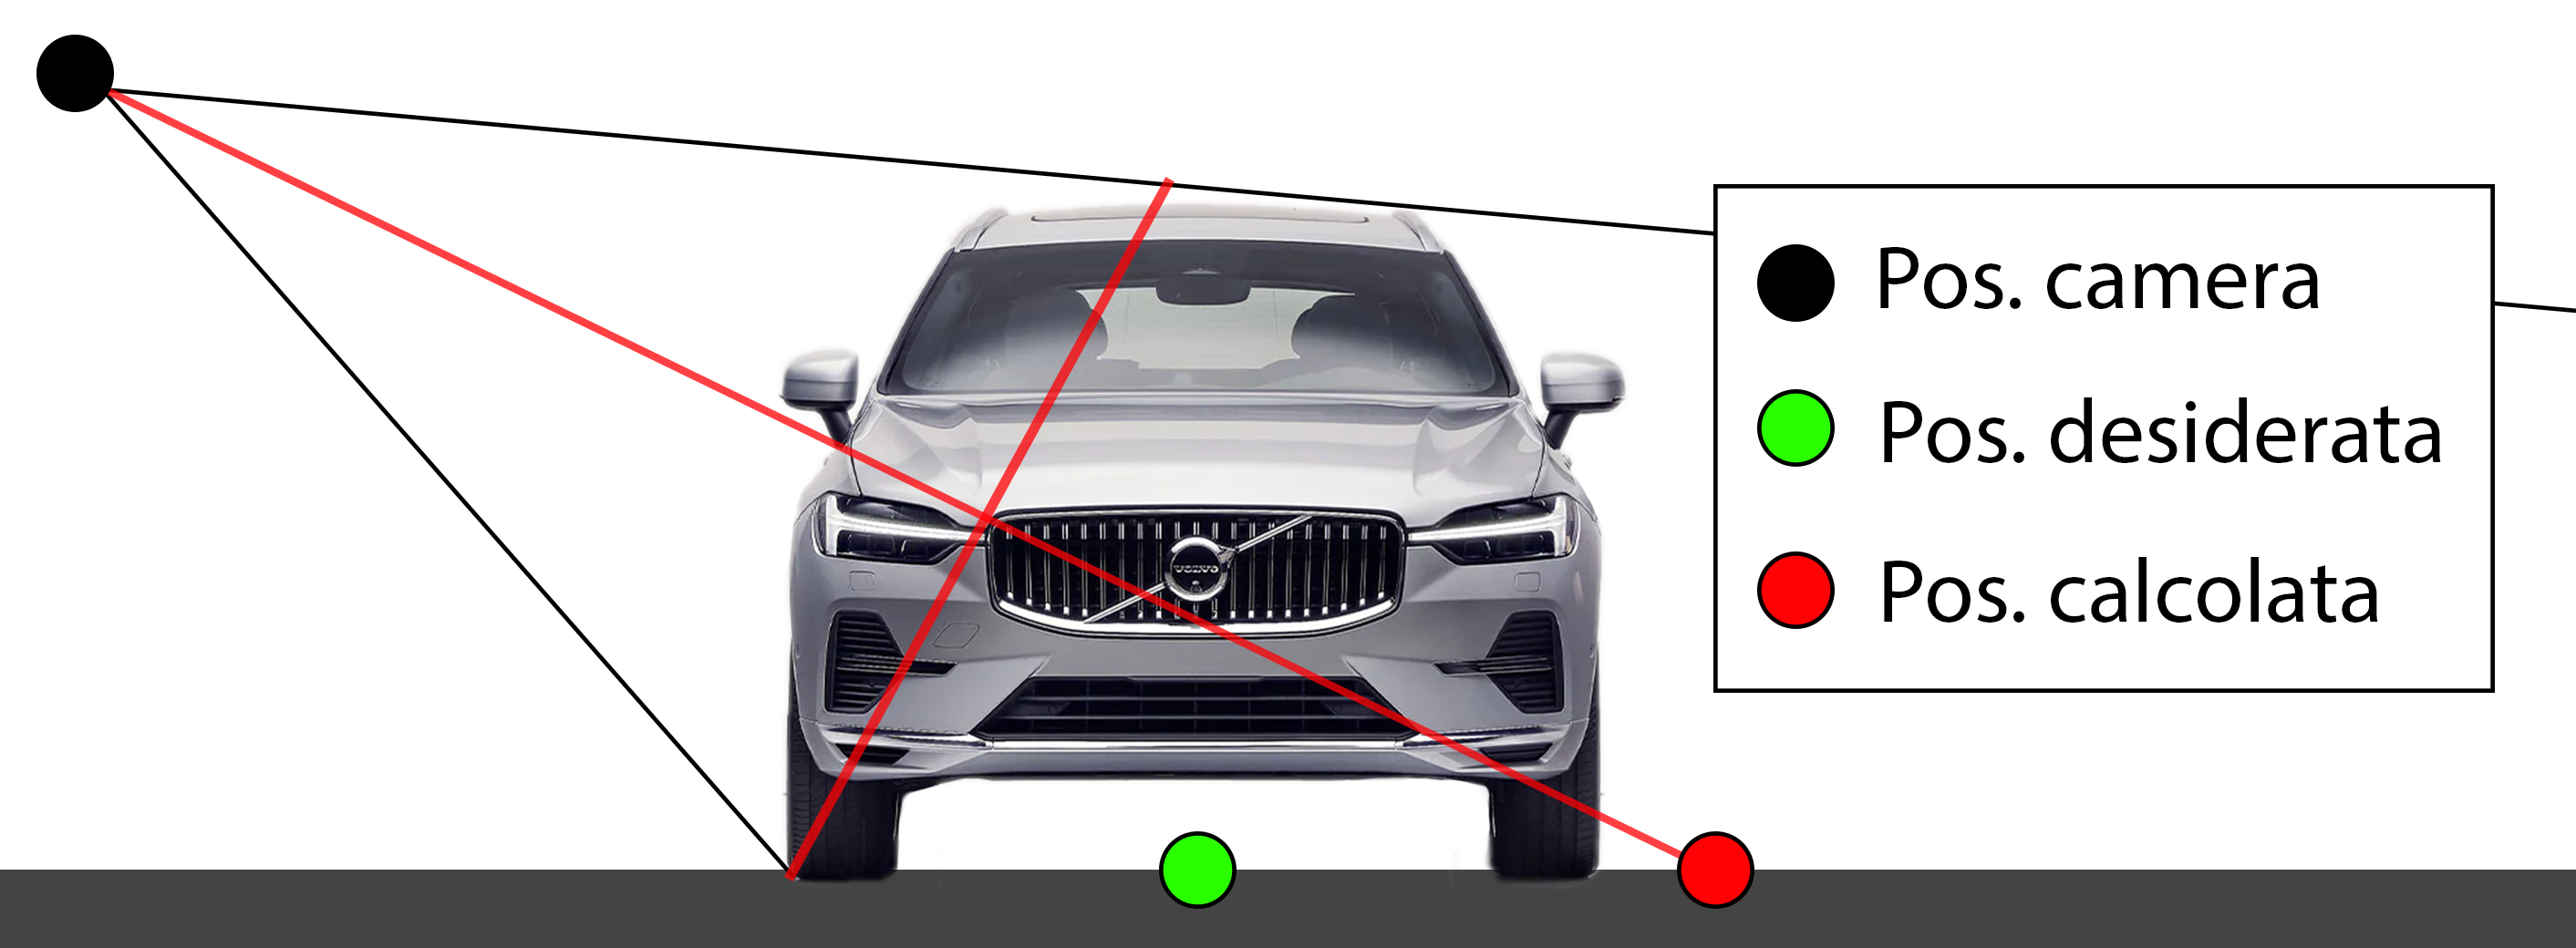
\includegraphics[width=\textwidth]{images/proiez_pos.png}
    \caption{Proiettare il centro dell'entità non da buoni risultati}
    \label{fig:proiezcenter}
\end{figure}

L'ultima considerazione necessaria è la scelta del punto a cui applicare la trasformazione trovata.
Notiamo dall'immagine \ref{fig:proiezcenter} che scegliere il punto centrale del Bounding Box non restituisce il risultato desiderato.
Un possibile approccio è quello di proiettare il lato inferiore del Bounding Box, in quanto questo è l'unico che poggia sul piano stradale.
Il centro delle entità può poi essere approssimato date le conoscenze relative a dimensioni medie della sua categoria, dalla sua direzione di movimento e dalle caratteristiche del Bounding Box.
Questa soluzione non è perfetta, ma i risultati ottenuti si sono dimostrati accettabili in fase sperimentale.

In fig \ref{fig:perspbbox} è presentata una scena annotata con Bounding Boxes.
In fig \ref{fig:perspcorrect} è presentata la stessa scena dopo che è stata eseguita la correzione della distorsione prospettica, in cui la posizione dei veicoli è indicata dal cerchio verde.

\begin{figure}[h]
    \centering
    \begin{subfigure}{.49\textwidth}
        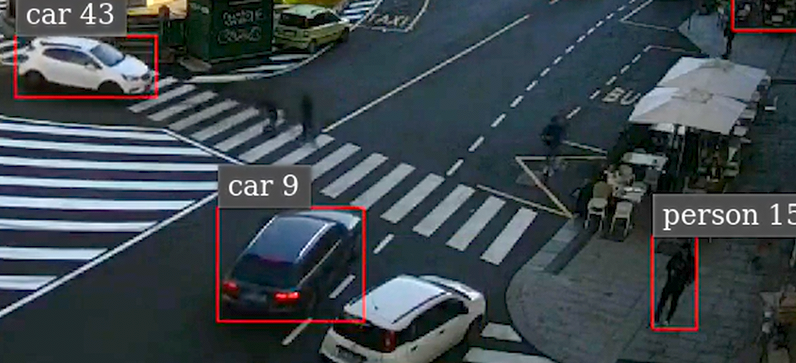
\includegraphics[width=\textwidth]{images/yolo.png}
        \caption{Bounding Boxes}
        \label{fig:perspbbox}
    \end{subfigure}
    \hfill
    \begin{subfigure}{.49\textwidth}
        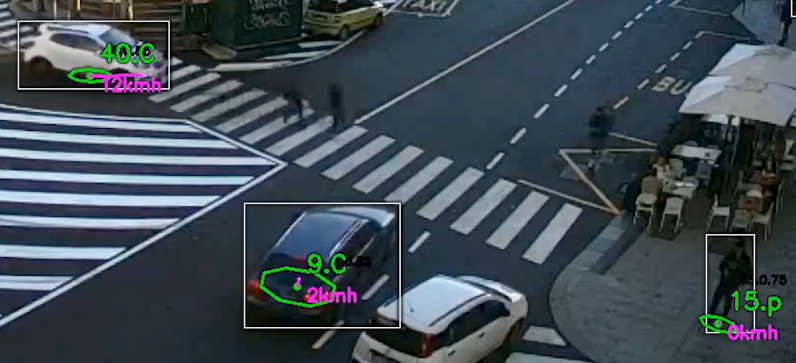
\includegraphics[width=\textwidth]{images/corrected.png}
        \caption{Prospettiva corretta}
        \label{fig:perspcorrect}
    \end{subfigure}
    \caption{Scena prima e dopo la correzione della distorsione prospettica}
\end{figure}
